\begin{frame}[fragile]
    \frametitle{Diferencia entre Git y Github}
        Git es un sistema de control de versiones distribuido, diseñado por
        Linus Torvalds, inicialmente para satisfacer las necesidades del
        Kernel de Linux, tras romper relaciones con la empresa que desarrollo
        su anterior herramienta (Bitkeeper).



Y qu\'e es Github? Es un hosting online para alojar repositorios que usan Git para el manejo del c\'odigo fuente.


\begin{figure}[t]
        \centering
        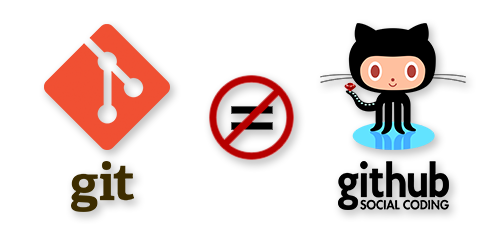
\includegraphics[width=0.5\textwidth]{Images/1.png}
\end{figure}


%Por tanto Git es algo m\'as general que nos ayuda a controlar el estado de un proyecto, Github es un sitio que usa Git en su funcionamiento.

\end{frame}
